\documentclass[a4paper,10pt, bibliography=totocnumbered]{scrreprt}

\usepackage[utf8x]{inputenc}
\usepackage[english]{babel}

\usepackage{graphicx}
\usepackage{pdfpages}
%\usepackage{subfig}
%\usepackage{microtype}
\usepackage{tabularx}
%\usepackage{amsmath, textcomp}

% Custom packages
\usepackage[numbers]{natbib}
\usepackage{longtable}
\usepackage{ragged2e}
%\usepackage{tikz}
%\usetikzlibrary{positioning}
%\usepackage{pdflscape}
%\usepackage{rotating}

\usepackage{glossaries} 

\usepackage{hyperref}
\hypersetup{
    colorlinks=true,        % false: boxed links; true: colored links
    linkcolor=black,        % color of internal links
%    citecolor=green,        % color of links to bibliography
    citecolor=black,        % color of links to bibliography
    filecolor=magenta,      % color of file links
    urlcolor=blue           % color of external links
}


%% Title Page
\makeatletter
\renewcommand{\maketitle}{\begin{titlepage}
    \vskip 10\p@
    \hbox{
      \vrule depth 0.99\textheight
        \mbox{\hspace{2em}}
      \vtop{
        \vskip 10\p@
        \hspace{4pt}
        \vskip 50\p@
        \begin{flushleft}
          \Large \@author \par
        \end{flushleft}
        \vskip 50\p@
        \begin{flushleft}
          \huge \bfseries \@title \par
        \end{flushleft}
        \begin{flushleft}
          \Large \bfseries \@subtitle \par
        \end{flushleft}
        \vskip 70\p@
        \begin{flushleft}
          \Large \@publishers \par
        \end{flushleft}
        \vskip 50\p@
        \begin{flushleft}
          \Large \@date \par
        \end{flushleft}
        }}
  \end{titlepage}
}
\makeatother

\author{Benjamin Tuna}
\title{Summarization in Bug Tracking Systems }
\subtitle{ }
\publishers{\textbf{Advisor University of Heidelberg}\\ Prof. Dr. Barbara Paech, Marcus Seiler}
\date{01 31, 2022}



% Deutsche Absaetze:
\parindent 0pt
\parskip 12pt

\textwidth145mm
\setlength{\oddsidemargin}{0.7cm}
\setlength{\topmargin}{-0.5cm}
\setlength{\textheight}{22.5cm}

\begin{document}
\maketitle

\include{./content/0-Abstract}

\tableofcontents

\chapter{Introduction}


This paper examines approaches to summarizing bug reports and their efficiency for the developers and managers of a software project. It often happens that a bug report is written more than once. This leads to confusion of the employees as well as to complications in the software cycle. The first paper ''Automated Summarization of Bug Reports to speed-up software development/maintenance process by using Natural Language Processing (NLP)'' by Tarar et al. \cite{tarar} which is described in the following, deals with the question whether it is possible to generate a summary of bug report automatically and the use of it is also meaningful. Thereby methods like Natural Language Tool Kit (NLTK), Skipt-thought, K-Mean-Cluster, TF-IDF are used for the execution of the algorithm. NLTK is a tool that is responsible for the preparation of a text and simplifies the implementation through natural language. The sentences from a bug report are computed into vectors using Ski-thought and then divided into clusters containing similar sentences using K-Mean-Cluster. TF-IDF can then be used to calculate the extent to which a sentence is significant and meaningful. The second paper ''Bug Report Summarization using Believability Score and Text Ranking'' by Koh et al. \cite{koh} is very recent and is ready to address the question of how to improve the summary quality of such a methodology. Here it is mainly about the Believability Score which is combined with the Text Ranking. The Believability Score is a number that indicates how credible a bug report is based on the comments. The Text Ranking then happens by determining the equality of sentences based on their meaning and assigning a rank. 
\linebreak
In chapter \ref{literatur} the procedure of the literature search is described and how the selection of the papers was done. In chapter \ref{approach1} the first paper is explained and in chapter \ref{approach2} the second paper. After that, in chapter \ref{comparison} the synthesis is described and a comparison is given. The last chapter \ref{conclusion} is a conclusion.




\chapter{Literature Search}
\label{literatur}
%Vorgehen der Literatursuche
	%Forschungsfragen: Wie werden Bug Reports zusammengefasst und 						wie effizent ist deren Nutzung
			
	%Relevanzkriterien: 
		%Artikel beschreibt Ansatz zur Zusammenfassung von Bug 					Reports
		%Artikel zeigt Ergebnis seiner Methode
		%Artikel sollte nicht älter als 10 Jahre sein
		%Englisch
		%Nicht die selben AutorInnen
To find appropriate articles for this paper, a literature search was conducted to explore methods for summarizing bug reports. Prior to the search, relevance criteria were defined by the author and the instructors to achieve a successful search. First, the article should describe an approach to summarizing bug reports and illustrate its results. Due to the constantly evolving nature of software, the date of publication of the article should not be more than 10 years in the past. Since an English article is to be written as part of the seminar, the language of study is English, and most papers on the subject are written in English, it was specified that the paper to be found should also be in English. A paper to investigate the research question has already been given by the lecturers. So, to get a balanced result it was also assumed that the authors are not the same. For the search of the second paper, two methods were used and then the results of the search were compared to find a suitable paper.
\section{Search Methodic}
%Suchemethodik
Since the search for paper can sometimes be endless and one can lose track of a large number of hits, the snowballing method was used on the one hand and a search term based search on the other. 
\subsection{Snowballing}
Snowballing is a method that performs a literature search based on a finished article. All articles cited by the authors and cited by other articles are examined. If the articles that cite the given article are examined, it is called forward snowballing. Examining the articles that cite the authors of the given article is called backward snowballing.
\subsubsection{Forward Snowballing}
In Forward Snowballing, 215 articles were found, of which only one was linked. This article was about classifying people to analyze mental health related to social media, which was not relevant for the here explored topic.


\subsubsection{Backward Snowballing}

In Backward Snowballing 27 articles were found. First, the headings of the articles were taken into account and thus already the non-relevant papers were excluded. Then four papers remained, whose abstract and introduction were read and why they were relevant or not relevant was documented in Table \ref{tab:backward}. 

\begin{table}
\begin{tabular}[h]{p{3cm}|p{3cm}|p{3cm}|p{3cm}}
Name & Date & Relevant (yes/no) & Explanation \\
\hline
Hipikat: recommending pertinent software development artifacts & 05.11 & yes & a tool that builds a group memory from the project to suggest to a newcomer what he needs to work on a task. \\
\hline
Towards more accurate retrieval of duplicate bug reports & 05.11 & yes & Measure and summarize similarities between defect reports to improve the process \\
\hline
Automatic Summarization of Open-Domain Multiparty Dialogues in Diverse Genres & 05.11 & no & Here the merging of dialogs is considered, but it is only about speech recognition and not primarily about bug reports  \\
\hline
Communication, collaboration, and bugs: the social nature of issue tracking in small, collocated teams & 05.11 & no & Here, the importance of issue trackers is explored but not the simplification through the aggregation of issues \\
\end{tabular}
\caption{Results of backward Snowballing}
\label{tab:backward}
\end{table}

\subsection{Searcterm based Search}
In the search term based search, searches are performed on various libraries using terms. The search libraries used are IEEE, ACM, Springer and ELSEVIER on the recommendation of the lecturers. The number of papers found as a function of the search terms was then noted and thereupon those of relevance were sorted out from those that were not. Relevance was again determined by reading the abstract and introduction. If a search yielded no relevant results, the reason was noted.
The searches for this article can be found in Table \ref{tab:searchterm}.

\begin{table}
\begin{tabular}[h]{p{1cm}|p{1cm}|p{2cm}|p{2cm}|p{1cm}|p{1cm}|p{3cm}}
Webpage & Date & Search limitation & Result & Relevant result & Comment \\
\hline
IEEE & 05.11 & Date: 2012-2022 & Bug Tracker AND Summarization & 2 & 0 & Here it was more to the simplification of software process and not about bug tracker or bug reports  \\
\hline
IEEE & 05.11 & Date: 2012-2022 & Bug Reports AND Summariz ation AND Automated & 7 & 4 & - \\
\hline
ACM & 05.11 & Date: 2012-2022 in Astract ''Bug Reports'' AND Summarization &  ''Bug Reports'' AND Summarization AND Automated & 14 & 3 & - \\
\hline
ACM & 05.11 & Date: 2012-2022 in Astract ''Bug Reports'' AND Summarization &  Bug Tracker AND Summarization AND Automated & 104 & 0 & Here it went again primarily about the automation and simplification from software processes and not special about bug reports\\
\hline
Springer & 05.11 & Date: 2012-2022 &  ''Bug Reports'' AND Automated AND Summarization & 101 & 3 & -\\
\hline
ELSEVIER & 05.11 & Date: 2012-2022 &  Bug Reports AND Summarization AND Automated & 5696 & 0 & No articles that occupy
with my topic\\
\hline
ELSEVIER & 05.11 & Date: 2012-2022 &  Bug Tracker AND Summarization AND Automated & 2871 & 0 & No articles that occupy
with my topic\\
\end{tabular}
\caption{Results of Search term based search}
\label{tab:searchterm}
\end{table}


Since some articles overlapped, the following relevant articles have been documented as a result (see Table 4).
\section{Results}
%Ergebnisse der Suche(Statistiken, Suchtabelle, Ausgewählte Arbeiten)
The results of both search methods were then summarized. The name of the paper, keywords used in the paper, a short motivation, the research question of the paper, the basic idea of the paper, a summary of the paper and a short comment on the paper were noted. These points then helped in the selection of the paper.
\linebreak

The paper "Bug Report Summarization using Believability Score and Text Ranking" \cite{koh} was the only one that was completely different in method from the given paper. It follows an interesting and new approach to summarization of bug reports.


\chapter{Approach : Automated Summarization of Bug Reports to speed-up software development/maintenance process by using Natural Language Processing (NLP)}
\label{approach1}

		%Thema 1: ob es möglich ist, die Fehlerberichte so 						zusammenzufassen, dass sie für Entwickler 							während des Entwicklungsprozesses nützlich sind
		


\section{Goal}
The authors of \cite{tarar} define the goal of this article as investigating whether it is possible to summarize bug reports in such a way that they are useful for developers during the development process. For this purpose, an algorithm was proposed by the authors, which was then compared with a Golden standard summary. The Golden Standard Summary is a Summary that was createt from people to compare the results of the Method \cite{tarar}.
\section{Algorithm}
In the algorithm, the similarity between sentences is calculated. The sentences are converted into vectors and then clustered. Then the sentences within a cluster are ranked and the sentence with the highest rank is used for the summary. For the implementation of the algorithm Python was used. The individual steps of the algorithm are explained in the following subsections.
\subsection{Pre-Processing}
Natural Language Tool Kit(NLTK) is used to first combine all records of the given documents such as bug reports or from CSV files. NLTK is a tool that allows the user to write a Python program in natural language. For the combination of the sentences first stop words are removed and stemming is performed. Then the string data is tokenized and these sentences are written to a list. These prepared sentences are packed into vectors in the next step. How the code in NLTK looks like or works in detail is not explained further.
\subsection{Sentence Embedding}
In this step, the preprocessed sentences are packed into fixed-length vectors. For this, the authors use the so-called skip-thought method. Here, the words of a sentence are mapped as numbers in the sentence vector and then compared.
\subsection{Clustering Based on Similarity}
The words of the sentences are now compared within the vectors. K-Mean clustering is used for this purpose. It forms a predefined number of groups from all vectors that are similar. Accordingly, all sentences that are similar to each other are packed into a common cluster. To sort the sentences within the clusters, a rank is assigned to them.
\subsection{Sentence Ranking}
TF-IDF is used for ranking. A word from the sentences is assigned a high weight if it occurs frequently in a single document or bug report but rarely in the entire collection of bug reports. If a term occurs in almost all bug reports in the collection, it is given a low weight. The reason for this is that a term that occurs in almost all Bug Reports, such as "a", does not give a distinctive weight to the Bug Reports. These are also often stop words. So to calculate the weight, the frequency of a word in a Bug Report and the frequency of the word in the entire collection of Bug Reports is needed.  First, the inverse frequency of a word in the bug reports is calculated by \textbf{Figure \ref{fig:simi}}.

\begin{figure}
\centering
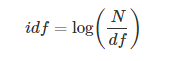
\includegraphics[scale=0.65]{../images/Thema10_idf.PNG}
\caption{inverse Frequency of a word}
\label{fig:simi}
\end{figure} 

Where N is the number of all error reports and df is the frequency of the error report in which a word occurs. This can now be used to calculate the weighting of a sentence. The formula for this is \textbf{Figure \ref{fig:sw}}.

\begin{figure}
\centering
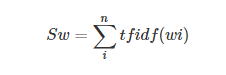
\includegraphics[scale=0.65]{../images/Thema10_Sw.PNG}
\caption{weighting of a sentence}
\label{fig:sw}
\end{figure} 

Here we iterate through all the sentences in a cluster. "n" is the number of all words within the sentence and wi is the i-th word of the sentence. Thus, the frequency of a word in a bug report is multiplied by the inverse frequency of a bug report in which the word occurs. The same calculation is performed only for each cluster. Then one more sentence is selected for display.
\subsection{Sentence Selection}
Now that all sentences have been given a weight, one sentence from each cluster can be selected with the highest weight and placed at the top. Thus the redundancy is solved and the bug reports are summarized.

\section{Evaluation}
The algorithm explained above was implemented through the support of Theano. Theano is a Python-based library for computing mathematical expressions. This then converts the expressions into efficient executable code. The code can be executed quickly and transparently by both GPU and CPU.
For the evaluation of the described method, a standard data set also known as Summary Data Set (SDS) was implemented. The SDS contains 36 bug reports with a total of 2361 records. Each bug report was annotated by 3 people who wrote an abstract for each bug report. These summaries are described as Gold Standard Summaries and are used to evaluate the method developed in this paper. 
To compare the Gold Standard summary with the summary generated by the algorithm, a metric called ROUGE (Recall-Oriented Understudy for Gisting Evaluation) was used. ROUGE contains a number of metrics. However, ROUGE-1 and ROUGE-2 were used here. ROUGE-1 compares in a sentence the individual words from the summary generated by the method with the same sentence from the Gold Standard. For example, if the generated sentence is "I really interested about computer" and the sentence from the Gold Standard is "I interested about computer", the recall, precision, and F1 score are calculated. ROUGE-2 compares word pairs of the sentence in contrast to ROUGE-1. From the above example, here the pairs "I really", "really interested", "interested about" and "about computer" are made for the generated sentence. The same thing happens with the sentence from the Gold Standard. Now the word pairs are compared instead of each word and the recall and precision are calculated. After that, for the evaluation of the method, the average value of these calculations is taken and in Figure \ref{fig:eva1} it can be seen that Sentence embedding had the best values for ROUGE-1 and ROUGE-2 compared to other methods \cite{lin}.

\begin{figure}
\centering
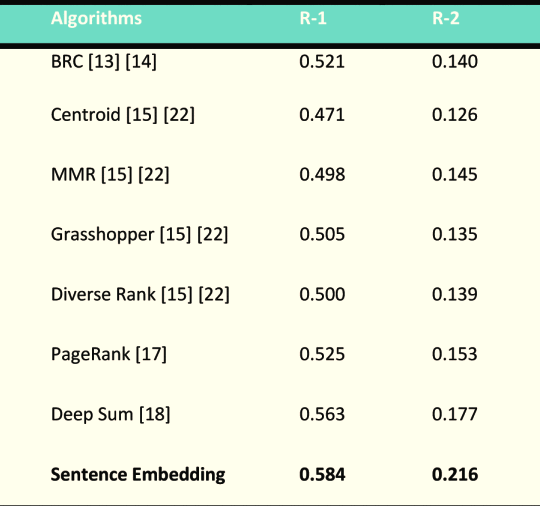
\includegraphics[scale=0.65]{../images/Thema10_ROUGE.PNG}
\caption{Result of ROUGE-1 and ROUGE-2}
\label{fig:eva1}
\end{figure} 

\section{Example}

To understand the above algorithm in more detail, here is a short example. 
As already described, the bug reports are first packed into the NLTK. Then, stop words like "too" are removed, since they often have no meaning for the understanding of the sentence. For example, the sentence "I like the food too" can be understood without the "too". Stemming is then performed, whereby words such as "eating", "eats" or "eaten" become "eat". After that the sentences are tokenized, unfortunately it is not explained how this is done. Now the sentences are packed into vectors. The words of the sentences are assigned a number, for example "I am the author" becomes [0.1, 0.2, 0.3, 0.4] and "The author is me" becomes [0.3, 0.4, 0.2, 0.1]. In the next step, similar sentence vectors are clustered. Before that, however, we compare which sentences are similar. In the example just shown, we can see that the sentences are identical, but in a different order, which indicates that the sentence is the same and thus are written into a common cluster. After that we calculate a rank of the sentence by TF-IDF. To do this, we first need the formula for determining the inverse frequency of a word in all bug reports (\ref{fig:simi}). The number of all bug reports should be 36 and the number of bug reports in which the word occurs should be six. Thus the inverse frequency would be 0.77815125038. To determine the weight we also need \textbf{Figure \ref{fig:eva1}}.
If now the word "Summarization" occurs five times in a bug report and the inverse frequency is 0.778 as calculated before, the result after one run would be 3.89 if the sentence contained only one word. If we now take a cluster as an example with 3 similar sentences, the sentence with the highest weight is chosen and the redundancy is solved. 

\chapter{Approach : Bug Report Summarization using Believability Score and Text Ranking}
\label{approach2}

		%Thema 2: Ist es möglich die Zusammenfassungsqualität von 				Bug Reports zu verbessern durch zuweisen eines 						Text Ranking scores Glaubwürdigkeitsscores für jeden 				Satz in einem Bug Report.
		
\section{Goal}
The aim of this article is to investigate whether the quality of the summary of bug reports can be improved by using a credibility score and text ranking score. The bug report is first prepared, then evaluated and finally summarized. 
\section{Algorithm}
The Koh et al \cite{koh} explain algorithm in four parts. The first part is the preprocessing, the secound is the sentence assignment and last the generation of the summary. These steps are explained in the following.
\subsection{Bug Report Preprocessing}
To prepare the bug report the bug reports are divided into smaller sentences depending on their punctuation, tokenized, stop words removed and porter stemming applied. 
\subsection{Metrics for Sentence Assessment}
\subsubsection{Believability Score Assignments}
First, all sentences are divided into two categories. First, there are comments that score sentences and second, sentences that are scored by comments. Sentences that are scored by comments are assigned a Bscore. For example, a sentence that contains no comments has a Bscore of one. In addition, an opinion score, also called OPscore, is distributed. This scores the opinion of the comment against the rated sentence. This is done by the support of a Support-Vector-Mashine(SVM) classifier. After that, the text ranking score is assigned for evaluation \cite{liu}.
\subsubsection{Text Ranking Score Assignments}
Using the pre-trained BERT model, a sentence vector is extracted from a sentence. In this process, a context of each word in the sentence is searched. Then, the cosine similarity between the sentence vectors is calculated using the following \textbf{Figure \ref{fig:simi}}

\begin{figure}
\centering
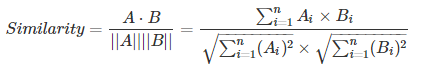
\includegraphics[scale=0.65]{../images/Thema10_Similarity.PNG}
\caption{Similarity between sentence vectors}
\label{fig:simi}
\end{figure} 

Cosine similarity determines the weight of similarity of two sentences. The frequency of a word in both sentences is taken and the more words match, the higher the similarity. Then, the TextRank score of a sentence is denoted by the following \textbf{Figure \ref{fig:textrank1}}.

\begin{figure}
\centering
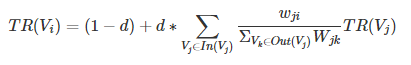
\includegraphics[scale=0.65]{../images/Thema10_textrank.PNG}
\caption{Rank of the sentence}
\label{fig:textrank1}
\end{figure}

To calculate the TextRank score now, we set the weight of cosine similarity for ''wij''. The sentence with the higher weight is the most important. The Text Rank is called Rscore. With this we have all the necessary information to create the summary

\subsection{Summary Generation}
The summary, also called Iscore, is calculated using the Bscore and Rscore (\textbf{Figure \ref{fig:iscore}}).

\begin{figure}
\centering
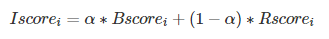
\includegraphics[scale=0.65]{../images/Thema10_iscore.PNG}
\caption{Calculate IScore}
\label{fig:iscore}
\end{figure}

Sentences that are supported by comments and sentences that are similar are important. Then the sentences are sorted and summarized according to the iscore.

\section{Evaluation}
The evaluation of this method was also performed by a Gold Standard Summary, which contains 36 sentences. The result of the method is measured by the metrics recall, precision and F-score. A calculation was performed for this using fixed weights but no implementation of the code. The calculations have shown that with a weight between 0 and 1, the combination of credibility score and text ranking returns better values for each metric than an already implemented tool called BugSum, which only works with the metric of credibility score (\textbf{Figure \ref{fig:ergebnisse}}). 

\begin{figure}
\centering
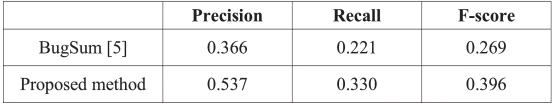
\includegraphics[scale=0.65]{../images/Thema10_ergebnisse.PNG}
\caption{Results of Method}
\label{fig:ergebnisse}
\end{figure}


\section{Example}
To make the above algorithm more understandable, an example of the individual steps is demonstrated here.
First, a sentence is divided into small sentences based on its punctuation marks. For example, the sentence "I'm studying at the university, that's where I'll graduate" is divided into the sentences "I'm studying at the university" and "That's where I'll graduate". According to which criteria tokenization is done is not listed by the authors. The stop words are also removed as already explained in the example from Approach 1. Subsequently, Porter stemming is performed. In Porter stemming, a word is stemmed back to the shortest form of the word. For example, the words Connect, Connection, Connections are traced back to Connect. A distinction is then made between the report sentences and comments. The Bug Report sentences are then given a credibility score which is calculated by multiplying the number of comments by an opinion score. The assignment of the opinion score is supported by the SVM classifier. SVM takes a sentence as input and predicts the probability of a negative opinion with a value between 0 and 1, drawing on the large amount of pre-trained data in the SVM classifier. Thereupon, the sentences are assigned a rank that corresponds to the Rscore. To do this, a sentence vector is first extracted from each sentence. For example, if "Hello" in BERT knows a context with "you", a vector is formed from it. Then the cosine similarity between two sentences is calculated. For example, if one sentence is "Me and my friends are drinking water" and the other is "My family and me are drinking water", we have found "me", "my", "are", "drinking" and "water" as common. The order does not matter here. Due to the amount of overlapping words, the Similarity value is high and the similarity of these two sentences is given. 

\chapter{Comparison}
\label{comparison}
\section{Summary}
The first paper is called "Automated Summarization of Bug Reports to speed-up software development/maintenance process by using Natural Language Processing (NLP)" by Tarar et al. \cite{tarar}, is using an extractive process. The goal of this paper is to find out if it is possible to summarize bug reports in a way that is useful for developers during the development process. In doing so, NLTK is first used to prepare the bug reports in order to separate and simplify the individual sentences and prepare them for further processing into vectors. Then, by using Skip-thought, the prepared sentences are packed into vectors and each word of a sentence is assigned a number in the process. In the next step, clusters of the sentences are formed. For this, first all the words within the vectors are checked for similarity by using K-Mean cluster and the sentences which have similarity are packed into the same cluster.  Then, a rank is assigned to the sentences by using TF-IDF. The sentence from each cluster with the highest rank is then displayed, thus resolving the redundancy of sentences from a cluster that are similar. This method was then evaluated by the ROUGE metric. This compared recall, precision, and F-score for the sameness of a Gold Standard sentence to the generated sentence from the method. The second paper "Bug Report Summarization using Believability Score and Text Ranking" from Koh et al. \cite{koh} addresses the question of whether it is possible to improve the summary quality of bug reports. Again, the bug reports are prepared first. The sentences are separated by punctuation, tokenized, stop words are removed and Porter stemming is performed. Next, a credibility score is calculated. Here, a prebuilt library analyzes contexts of words and comments of a bug report to define credibility. Then, a rank is calculated for the bug report by using TextRank. The bug reports are checked for similarity and receive a rank that indicates how meaningful a bug report is. Now, depending on the credibility score and the text ranking, it is calculated which sentence of those that are similar is the one with the highest credibility and has the highest rank and this is then chosen for the summary.

\section{Synthesis}

The method of Tarar et al. \cite{tarar} combines the files and removes the stop words and creates the root words. Then the character strings are tokenized in order to list all sentences. After that the generated sentences are converted into vectors of real numbers by sentence embedding. Then the sentences are wirtten into a sentence vector. Clustering is then carried out, whereby the features of the vectors formed are compared with one another and divided into clusters. From this, records are sorted according to information. The term weighting method assigns a weight to each sentence. Those sentences with a high rank are important for the ranking because they are shown. In order to be able to use this, the term frequency and document frequency are calculated in advance. Since the clusters with the similar sentences are now formed, each cluster is iterated and each stop word with low weight and the word stems are removed. A sentence with the highest weight comes out of each cluster and the redundancy has been resolved. Then the sentences are put in a new order. This approach was evaluated using a method that compares the automatically generated summaries with gold standard summary.
To evaluate, the result of the method of Tarar et al. \cite{tarar} was compared word by word with the Gold Standard Summary and the recall, precision and F-score were calculated. On average, these results yielded a precision of 0.584, where one would be the optimum. In addition, word pairs were compared with the Gold Standard Summary, with which the recall and precision were calculated and resulted in an average accuracy of 0.216, which is also the best value. \linebreak

In the method of Koh et al. \cite{koh} code snippets and stack traces are removed and divided into individual sentences using punctuation marks, and each sentence is tokenized according to regular expressions. Here, stop words are removed and porter stemming is carried out too. To evaluate the meaning of a sentence, the Believability score and the text ranking algorithm are used. For the Believability assessment, sentences are divided into two categories. There are sentences that are evaluated by other sentences (bug report) and sentences that evaluate others (comments). A rated set is assigned a Believability rating depending on the rating set. The opinion score then evaluates the opinion of the sentences that evaluate a sentence in comparison to the sentence that is evaluated. Then a prediction is made of the opinion with a value between zero and one. However, if a sentence that is evaluated is present, the Believability is calculated as a function of its evaluator sentences. The other metric mentioned earlier is the Text Ranking Score. A sentence vector is extracted from a sentence with subsequent calculation of the cosine similarity between the sentence vectors. A set with a high ranking score is then the most important of each vector. Finally, a collection of important sentences is carried out. Below are those sentences that are supported by other comments and are similar to others. This approach was evaluated by calculating the recall, precision and F-Score from a gold standard summary. The results were compared with one other tool and it was found that a combination of Believability and Text Ranking produces better and more accurate results. \linebreak

The goal of Tarar et al. \cite{tarar} was to show that bug reports can be summarized and have a benefit for developers and managers. Based on the results, it can be said that very good values are already achieved, but can still be improved. The goal of Koh et al. \cite{koh} was to improve the summary quality. The method was only compared with a tool, which also has worse values. However, considering that the first approach of Tarar et al. \cite{tarar} is already one year older and can show almost the same results or even better then the Method of Koh et al. \cite{koh}. Additionally Tarar et al. \cite{tarar} implemented their approach and Koh et al. \cite{koh} have not.


\section{Synthesis Matrix}

\begin{table}
\begin{tabular}[h]{p{3cm}|p{5cm}|p{5cm}}
Name & Automated Summarization of Bug Reports to speed-up software development/maintenance process by using Natural Language Processing (NLP) & Bug Report Summarization using Believability Score and Text Ranking \\
\hline
Used Methods & NLTK, Skip-thought, K-Mean-Cluster, TF-IDF & SVM, Believability-Score, Text Ranking \\
\hline
Classification Goal & better overview of Bug Reports & better overview of Bug Reports \\
\hline
Data requirements and limitations & Words must be assignable to different weights & Punctuation marks available, classification into different rankings \\
\hline
Supported Development Processes & Development process, documentation within a process, overview of bug reports
 & Development process, documentation within a process, overview of bug reports
 \\
\hline
Supported Stakeholders & Developer and Manager & Developer and Manager \\
\hline
Tool support / Prototype & Theano & none \\
\hline
Degree of Automation & Fully automatic & Fully automatic \\
\hline
Evaluation & "Recall-Oriented Understudy for Gisting Evaluation" ROUGE
 & recall, precision, F-Score \\
\hline
Evaluationresults & Summary possible, better results than other methods & Improvement of quality compared to BugSum but no better results than the first approach \\
\end{tabular}
\caption{Sysntesis Matrix}
\label{tab:matrix}
\end{table}


\section{Differences and Similarities}
Here the approaches are going to be compared based on the Synthesis Matrix \ref{tab:matrix}. Both approaches have the goal of summarizing bug reports and thus providing a better overview of bug reports. They initially divide the sentences in order to be able to examine them later. The approach of Tarar et al. \cite{tarar} inserts the sentences into vectors, which are compared and formed clusters of similar sentences. The sentences are then prioritized and assigned to a rank. The other approach of Koh et al. \cite{koh}, on the other hand, predict the believability and creates a text ranking. It examines how often a sentence was rated by other sentences and then classified due to the importance. In the first approach, stop words are removed and stemming is carried out, whereby a sentence with the highest weight is selected from each cluster and thus the redundancy is removed. In the second approach, a score is calculated from the believability and text ranking.

\chapter{Conclusion}
\label{conclusion}
In the approach of Tarar et al. \cite{tarar}, which is from 2020 and is one year older than the approach of Koh et al. \cite{koh}, the algorithm is described in more detail. The reason for this is that Tarar et al. \cite{tarar} developed a new approach and also implemented the method, where as Koh et al. \cite{koh} only made a change to existing approaches. Tarar et al. \cite{tarar} compares sentences by converting them into numbers then checks the similarity of these numbers to generate a summary of bug reports. Koh et al. \cite{koh} uses pre-trained libraries to calculate a credibility score by predicting a believability score and looking for connections in sentences to rank them.

%% Bibliography
\bibliographystyle{plainnat}
%\bibliography{literature.bib}%Bibliography file name

\begin{thebibliography}{9}

\bibitem{tarar} Nawaz Tarar, M. Irtaza / Ahmed, Faizan / Butt, Wasi Haider : Automated Summarization of Bug Reports to speed-up software development/maintenance process by using Natural Language Processing (NLP) In: 15th International Conference on Computer Science Education (ICCSE) p. 483-488 (2020)

\bibitem{koh}Koh, Youngji / Kang, Sungwon / Lee, Seonah : 
Bug Report Summarization using Believability Score and Text Ranking
In: International Conference on Artificial Intelligence in Information and Communication (ICAIIC) p. 117-120 (2021)

\bibitem{liu} Liu, Haoran / Yu, Yue / Li, Shanshan / Guo, Yong / Wang, Deze / Mao, Xiaoguang 
Bugsum: Deep context understanding for bug report summarization  
Proceedings of the 28th International Conference on Program Comprehension (2020)

\bibitem{lin}Lin, Chin-Yew 
Rouge: A package for automatic evaluation of summaries  
Text summarization branches out p. 74-81 (2004)


\end{thebibliography}

\listoffigures

\listoftables

\end{document}          
